% Modelo da UFMG -
% Este modelo foi baseado em: modelo-ufpr.tex,v 1.1 2003/06/30 15:05:18 gweber Exp $
% $Id: modelo-ufpr.tex,v 1.1 2003/06/30 15:05:18 gweber Exp $
%   Licence: LPPL (LaTeX Project Public License)
%     You can change this file in the terms of LPPL
%     (http://www.latex-project.org/lppl.html)
% copyright Rogério C. <rogerioc@cesec.ufpr.br>
%
% ****** DEFINIÇÕES INICIAIS ******	
\documentclass[a4paper,12pt, normaltoc, pnumromarab, pagestart=introducao, tocpage=plain]{abnt}
% Utilize a opção normalfigtabnum para numerar as figuras e tabelas por capítulo
%\usepackage[alf]{abntcite} chamada de referencia alfabetica
\usepackage[num]{abntcite}
\usepackage[brazil]{babel}
\usepackage[utf8]{inputenc}
\usepackage[T1]{fontenc}
\usepackage{indentfirst}
\usepackage{graphicx}														%Package para figuras
\usepackage{float}
\usepackage{geometry}
\geometry{a4paper,left=3cm,right=2cm,top=3cm,bottom=2cm}

%%
%%	Ainda em teste
%%
%\usepackage[bookmarks=false]{hyperref}					%Package para hyper-referências
%\hypersetup{colorlinks,
%							citecolor = black,
%							filecolor = black,
%							linkcolor = black,
%							urlcolor  = blue,
%						pdfnewwindow}
%
% O problema ocorre quando há referências do tipo \cite{} e \citeonline{}
% Há ainda outros problemas -> o figura, antes do número, não altera de cor na lista de figuras.
% O mesmo ocorre na lista de tabelas.
% O sumário aponta para a capa, não para o resumo, lista, apêndices ou anexos correspondentes.
% -> Funciona para capítulos.
%

\makeatletter	%Para que ele entenda o @

% Altera o tamanho das fontes dos capítulos e dos apêndices
\renewcommand{\ABNTchapterfont}{\bfseries}
\renewcommand{\ABNTchaptersize}{\Large}
\renewcommand{\ABNTanapsize}{\Large}

%Altera o espaçamento entre dots
%\renewcommand\@dotsep{2}

%Altera forma de montagem do table of contents
\renewcommand\l@chapter[2]{
  \ifnum \c@tocdepth >\m@ne
    \addpenalty{-\@highpenalty}%
    \vskip 1.0em \@plus\p@
    \setlength\@tempdima{1.5em}%
    \begingroup
      \ifthenelse{\boolean{ABNTpagenumstyle}}
        {\renewcommand{\@pnumwidth}{3.5em}}
        {}
      \parindent \z@ \rightskip \@pnumwidth
      \parfillskip -\@pnumwidth
      \leavevmode \normalsize\ABNTtocchapterfont
      \advance\leftskip\@tempdima
      \hskip -\leftskip
      #1\nobreak\dotfill \nobreak%
      \ifthenelse{\boolean{ABNTpagenumstyle}}
         {%
          \hb@xt@\@pnumwidth{\hss
            \ifthenelse{\not\equal{#2}{}}{{\normalfont p.\thinspace#2}}{}}\par
         }
         {%
          \hb@xt@\@pnumwidth{\hss #2}\par
         }
      \penalty\@highpenalty
    \endgroup
  \fi}

\renewcommand*\l@section{\@dottedtocline{1}{0em}{2.3em}}
\renewcommand*\l@subsection{\@dottedtocline{2}{0em}{3.2em}}
\renewcommand*\l@subsubsection{\@dottedtocline{3}{0em}{4.1em}}

% Cria um comando auxiliar para montagem da lista de figuras
\newcommand{\figfillnum}[1]{%
  {\hspace{1em}\normalfont\dotfill}\nobreak
  \hb@xt@\@pnumwidth{\hfil\normalfont #1}{}\par}

% Cria um comando auxiliar para montagem da lista de tabelas
\newcommand{\tabfillnum}[1]{%
	{\hspace{1em}\normalfont\dotfill}\nobreak
	\hb@xt@\@pnumwidth{\hfil\normalfont #1}{}\par}

% Altera a forma de montagem da lista de figuras
\renewcommand*{\l@figure}[2]{
	\leftskip 3.1em
	\rightskip 1.6em
	\parfillskip -\rightskip
	\parindent 0em
	\@tempdima 2.0em
	\advance\leftskip \@tempdima \null\nobreak\hskip -\leftskip
	{Figura \normalfont #1}\nobreak \figfillnum{#2}}

% Altera a forma de montagem de lista de tabelas
\renewcommand*{\l@table}[2]{
	\leftskip 3.4em
	\rightskip 1.6em
	\parfillskip -\rightskip
	\parindent 0em
	\@tempdima 2.0em
	\advance\leftskip \@tempdima \null\nobreak\hskip -\leftskip
	{Tabela \normalfont #1}\nobreak \tabfillnum{#2}}

% Define os comandos que montam a lista de símbolos
\newcommand{\listadesimbolos}{\pretextualchapter{Lista de Símbolos}\@starttoc{lsb}}
\newcommand{\simbolo}[2]{{\addcontentsline{lsb}{simbolo}{\numberline{#1}{#2}}}#1}
\newcommand{\l@simbolo}[2]{
	\vspace{-0.75cm}
	\leftskip 0em
	\parindent 0em
	\@tempdima 5em
	\advance\leftskip \@tempdima \null\nobreak\hskip -\leftskip
	{\normalfont #1}\hfil\nobreak\par}

% Define o comando que monta a lista de siglas
\newcommand{\listadesiglas}{\pretextualchapter{Lista de Siglas}\@starttoc{lsg}}
\newcommand{\sigla}[2]{{\addcontentsline{lsg}{sigla}{\numberline{#1}{#2}}}#1}
\newcommand{\l@sigla}[2]{
	\vspace{-0.75cm}
	\leftskip 0em
	\parindent 0em
	\@tempdima 5em
	\advance\leftskip \@tempdima \null\nobreak\hskip -\leftskip
	{\normalfont #1}\hfil\nobreak\par}

% Define o tipo de numeração das páginas
%\renewcommand{\chaptertitlepagestyle}{plain}

% Altera a posição da numeração de páginas dos elementos pré-textuais
\renewcommand\pretextualchapter{
	\if@openright\cleardoublepage\else\clearpage\fi
	\pagestyle{\chaptertitlepagestyle}
	\global\@topnum\z@
	\@afterindentfalse
	\@schapter}

% Altera a posição da numeração de páginas dos elementos textuais
\renewcommand{\ABNTsectionmark}[1]{
	\ifthenelse{\boolean{ABNTNextOutOfTOC}}
		{\markboth{\ABNTnextmark}{\ABNTnextmark}}
		{\sectionmark{#1}
		\pagestyle{\chaptertitlepagestyle}}}

% Redefine o tipo de numeração das páginas
\renewcommand{\ABNTBeginOfTextualPart}{
	\renewcommand{\sectiontitlepagestyle}{plainheader}
	\renewcommand{\thepage}{\arabic{page}}
%	\setcounter{page}{1}
}

\makeatother

%Altera o tamanho do parágrafo
\setlength{\parindent}{1.5cm}

% ********************************
% ***** Início do Documento ******
% ********************************
\begin{document}

\begin{titlepage}
\begin{center}
Universidade Federal de Minas Gerais \\
Instituto de Ci�ncias Exatas \\
Departamento de Ci�ncia da Computa��o\\
\end{center}
\vfill

\begin{center}
%\hspace{.45\textwidth} % posicionando a minipage
\framebox[.8\textwidth][c]{
\begin{minipage}{.7\textwidth}
\begin{center}
\vspace{1cm}
\textbf{Gera��o Procedural e Visualiza��o de Terrenos e Planetas em Tempo-Real} \par
\vspace{2em}
por \par
\vspace{2em}
F�bio Markus Nunes Miranda\par
\vspace{2em}
Proposta de Projeto Orientado em Computa��o II \par
\vspace{1em}
\footnotesize{Apresentado como proposta de trabalho na disciplina de Projeto Orientado em Computa��o II do Curso de Bacharelado em Ci�ncia da Computa��o da UFMG} \par
\vspace{2em}
Prof. Dr. Luiz Chaimowicz\par
Orientador\par
\vspace{2em}
Carl�cio Cordeiro\par
Co-Orientador\par
\vspace{1cm}

\end{center}
Assinatura do aluno:\par
\vspace{2em}
Assinatura do orientador:\par
\vspace{2em}
Assinatura do co-orientador:\par

\begin{center}


\end{center}
\end{minipage}
}

\vfill
Belo Horizonte -- MG \\
2009 / 1� semestre
\end{center}
\end{titlepage}



%\sumario

\chapter{INTRODUÇÃO}

\section{Visão geral}

    Exemplo de uso de siglas:
    
    Os modelos como \emph{Capability Maturity Model Integration} (\sigla{CMMI}{Capability Maturity Model Integration}), usado para avaliação da qualidade de \emph{software} a partir da maturidade dos processos da organização, tem ganhado muita ênfase no contexto da tecnologia de processos de \emph{software}.

    Exemplo de uso de referências:
    
    A incorporação de um processo geralmente não acontece de imediato, logo depois do processo ser formalizado. As pessoas da organização podem apresentar certa resistência quanto a mudança de hábitos, considerando os passos recomendados pelo processo apenas uma burocracia sem nenhuma vantagem para o projeto \cite{Wilson2002}. 


\section{Objetivo, justificativa e motivação}





\chapter{REFERENCIAL TEÓRICO}


\section{Exemplo de figura}
 
    A Figura \ref{estruturaBPM}  mostra uma visão simplificada do funcionamento dos sistemas BPM.
    \begin{figure}[H]
        \centering
        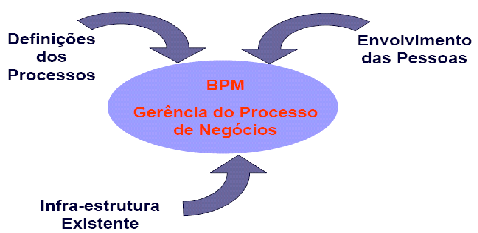
\includegraphics[scale=0.6,angle=0]{img/EstruturaBPM.png}
        \caption{Visão geral de um BPMS}
        \label{estruturaBPM}
    \end{figure}

\section{Exemplo de tabela}

	A Tabela \ref{tabFluxoUsa} mostra as atividades que compõem o fluxo de usabilidade e o papel requerido ao agente para realizá-las. As atividades de Análise de contexto de uso e Avaliação de usabilidade são decompostas em sub-fluxos, suas descrições são mostradas nas Tabelas \ref{tabAna} e \ref{tabAval}, respectivamente.

    \begin{table}[h]
        \begin{center}
    		\begin{tabular}{|c|c|}
    			\hline
                \textbf{Atividade} & \textbf{Papel requerido} \\ \hline
    			Planejamento & Gerente de Usabilidade \\
    			Controle  & \\
    			\hline
                Análise de contexto de uso &  \\
                Definição das funções do produto &  \\
                Prototipação de requisitos de interface & Analista de Usabilidade \\
                Definição de requisitos e metas de usabilidade & \\
                Revisão da análise de usabilidade & \\
                \hline
                Definição do estilo de interação & \\
                Desenho da interação & Arquiteto de usabilidade \\
                Revisão do desenho da interação & \\
                \hline
                Avaliação de usabilidade & Avaliador de Usabilidade  \\
                \hline
                Balanço final & Gerente de Usabilidade  \\
                \hline
    			%\multicolumn{3}{l}{\scriptsize Fonte: Indicar procedência.}\\
    			%\multicolumn{3}{l}{\scriptsize Notas: Alguma especificação geral.}\\
    			%\multicolumn{3}{l}{\scriptsize (1) Alguma nota específica}
    		\end{tabular}
    		\caption{Atividades do fluxo de usabilidade}
        	\label{tabFluxoUsa}
    	\end{center}
    \end{table}

    \begin{table}[h]
        \begin{center}
    		\begin{tabular}{|c|c|}
    			\hline
                \textbf{Atividade} & \textbf{Papel requerido} \\ \hline
    			Planejamento &  \\
                Preparação &  \\
                Modelagem preliminar de  usuários  &  \\
                Refinamento da modelagem de usuários &   \\
                Definição do modelo mental & Analista de Usabilidade  \\
                Análise de produtos concorrentes &  \\
                Modelagem preliminar de tarefas &  \\
                Refinamento da modelagem de tarefas &  \\
                Balanço final &  \\
                \hline
    			%\multicolumn{3}{l}{\scriptsize Fonte: Indicar procedência.}\\
    			%\multicolumn{3}{l}{\scriptsize Notas: Alguma especificação geral.}\\
    			%\multicolumn{3}{l}{\scriptsize (1) Alguma nota específica}
    		\end{tabular}
    		\caption{Atividades do sub-fluxo de análise de contexto de uso}
        	\label{tabAna}
    	\end{center}
    \end{table}

    \begin{table}[h]
        \begin{center}
    		\begin{tabular}{|c|c|}
    			\hline
                \textbf{Atividade} & \textbf{Papel requerido} \\ \hline
    			Planejamento &  \\
                Desenho &  \\
                Implementação &  \\
                Execução & Avaliador de Usabilidade  \\
                Análise dos dados &  \\
                Verificação do término &  \\
                Balanço final &  \\
                \hline
    			%\multicolumn{3}{l}{\scriptsize Fonte: Indicar procedência.}\\
    			%\multicolumn{3}{l}{\scriptsize Notas: Alguma especificação geral.}\\
    			%\multicolumn{3}{l}{\scriptsize (1) Alguma nota específica}
    		\end{tabular}
    		\caption{Atividades do sub-fluxo de avaliação de usabilidade}
        	\label{tabAval}
    	\end{center}
    \end{table}



\section{Metodologia}

\subsection{Metodologia}

\begin{frame}\frametitle{Metodologia} 
\begin{itemize}
	\item Livro \emph{Texturing and Modeling: A Procedural Approach} \cite{livro}.
	\item Estudo das melhoras formas de reduzir o gasta com mem�ria atrav�s de estruturas de dados do OpenGL.
	\item Estudo da arquitetura da \emph{GPU}.
	\item Implementa��o do sistema.
\end{itemize}
\end{frame}


\chapter{RESULTADOS E DISCUSS�O}
\label{resultados}
Neste cap�tulo, ser� apresentado algumas imagens de terrenos gerados (Se��o \ref{terrenosgerados}) e tamb�m algum testes executados (\ref{testes}).


\section{Terrenos gerados}
\label{terrenosgerados}

A Figura \ref{fig:heightmap2} mostra a renderiza��o de uma cena apenas com a textura do mapa de altura aplicado em um quadrado.
\begin{figure}[H]
	\center{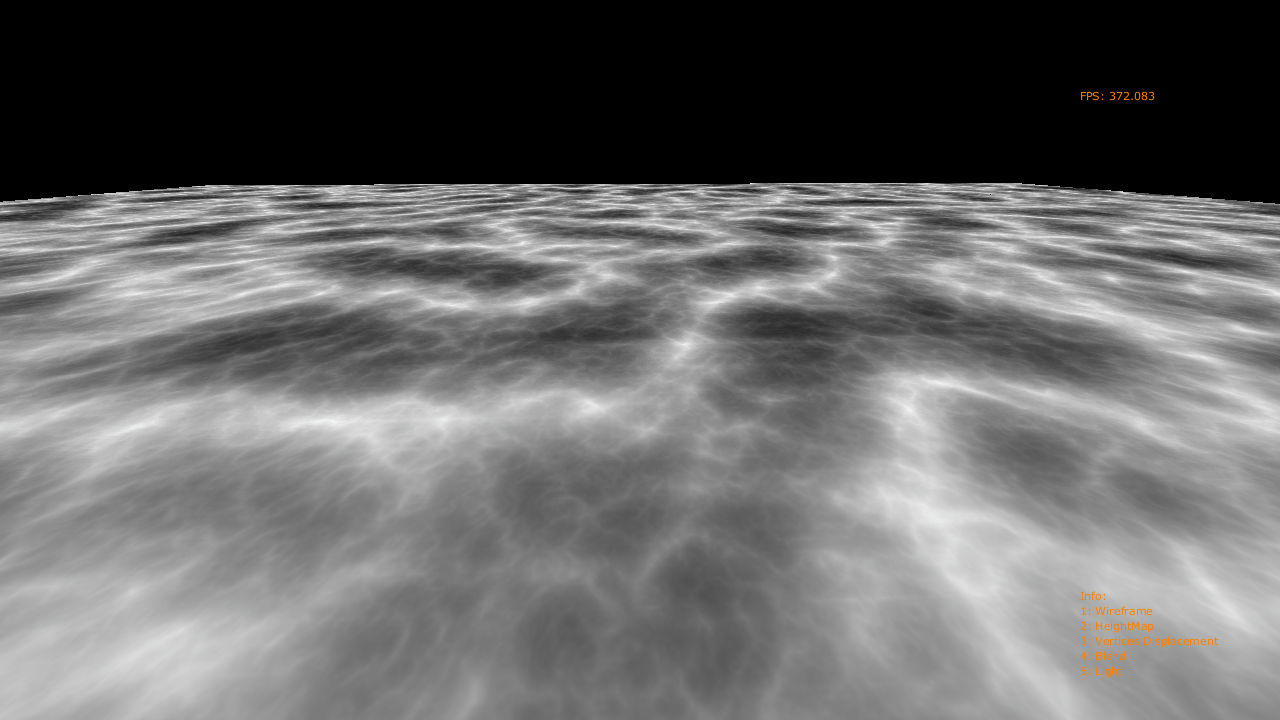
\includegraphics[width=0.5\linewidth]{img/caps/heightmap2.png}}
	\caption{\label{fig:heightmap2} Mapa de altura aplicado a um quadrado.}
\end{figure}


A Figura \ref{fig:deslocamento} mostra o mesmo mapa de altura, mas agora com o deslocamento dos v�rtices no eixo \emph{z}.
\begin{figure}[H]
	\center{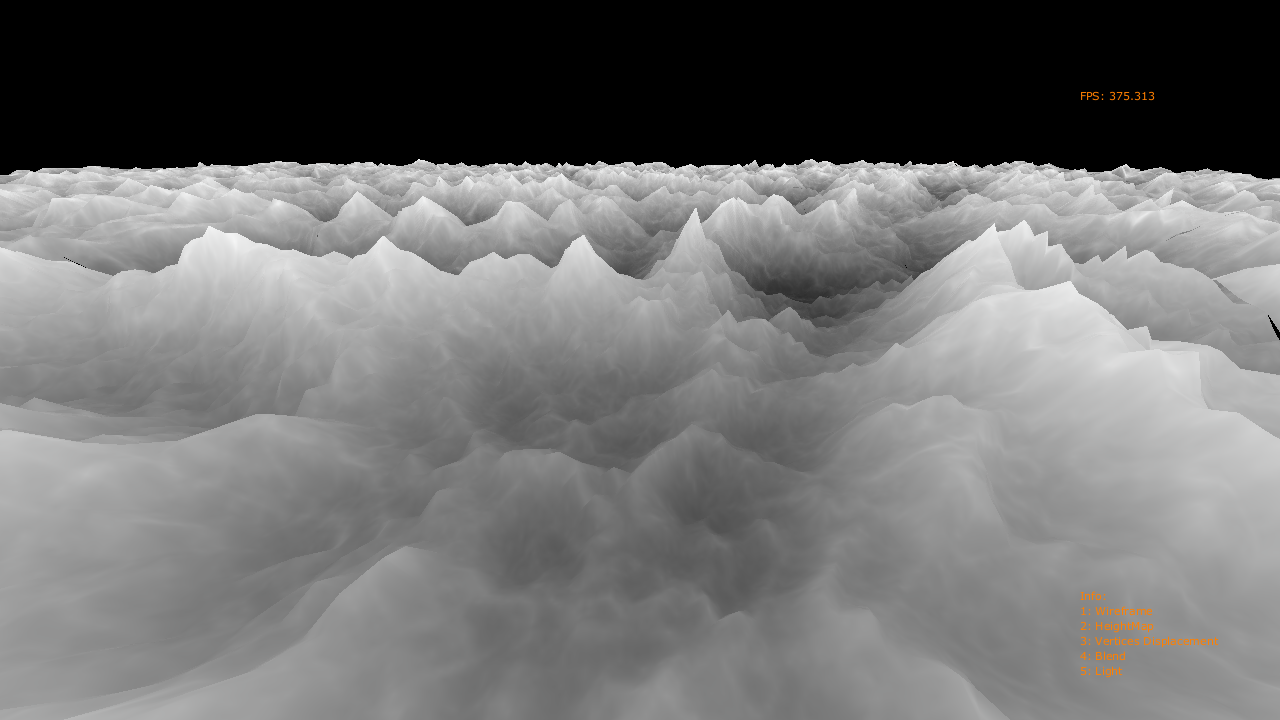
\includegraphics[width=0.5\linewidth]{img/caps/deslocamento.png}}
	\caption{\label{fig:deslocamento} Mapa de altura aplicado a um quadrado, deslocando a altura.}
\end{figure}

A Figura \ref{fig:blend} mostra agora a renderiza��o da malha com cores para simular grama, pedras, neve, etc.
\begin{figure}[H]
	\center{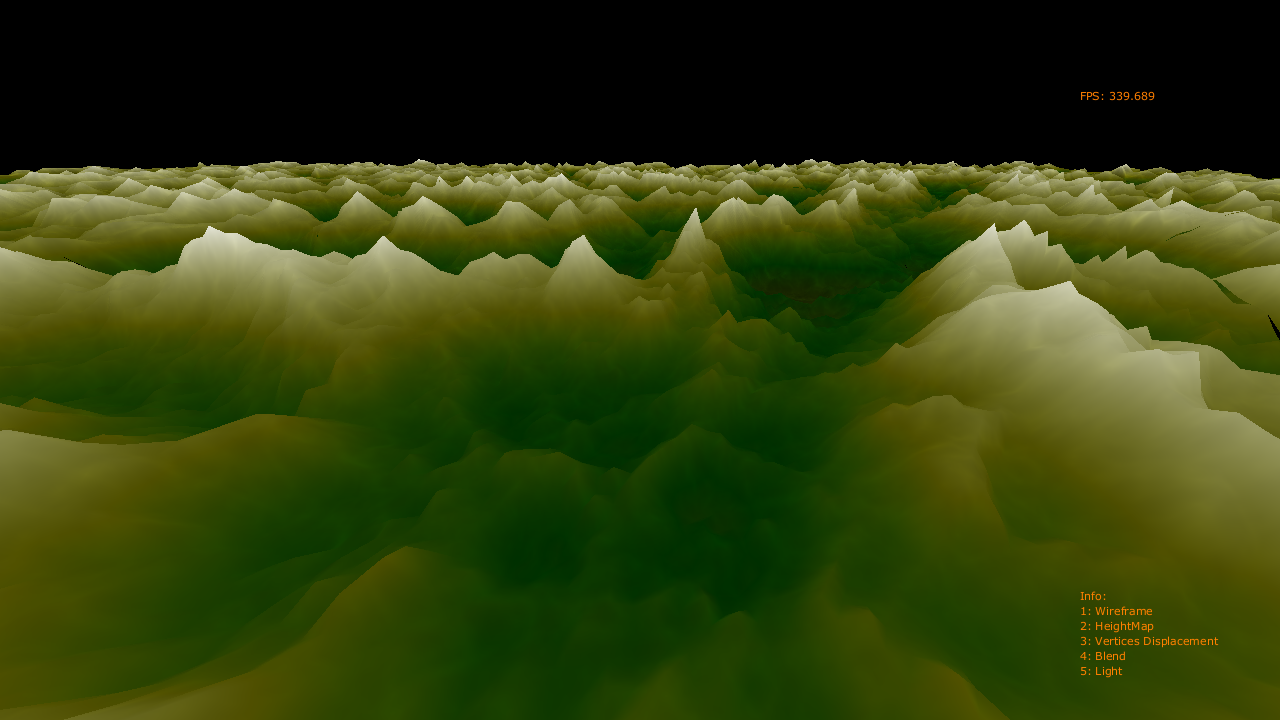
\includegraphics[width=0.5\linewidth]{img/caps/blend.png}}
	\caption{\label{fig:blend} Mapa de altura aplicado a um quadrado, deslocando a altura, e com texturas.}
\end{figure}

A Figura \ref{fig:luz} mostra o resultado final, agora com a aplica��o de ilumina��o.
\begin{figure}[H]
	\center{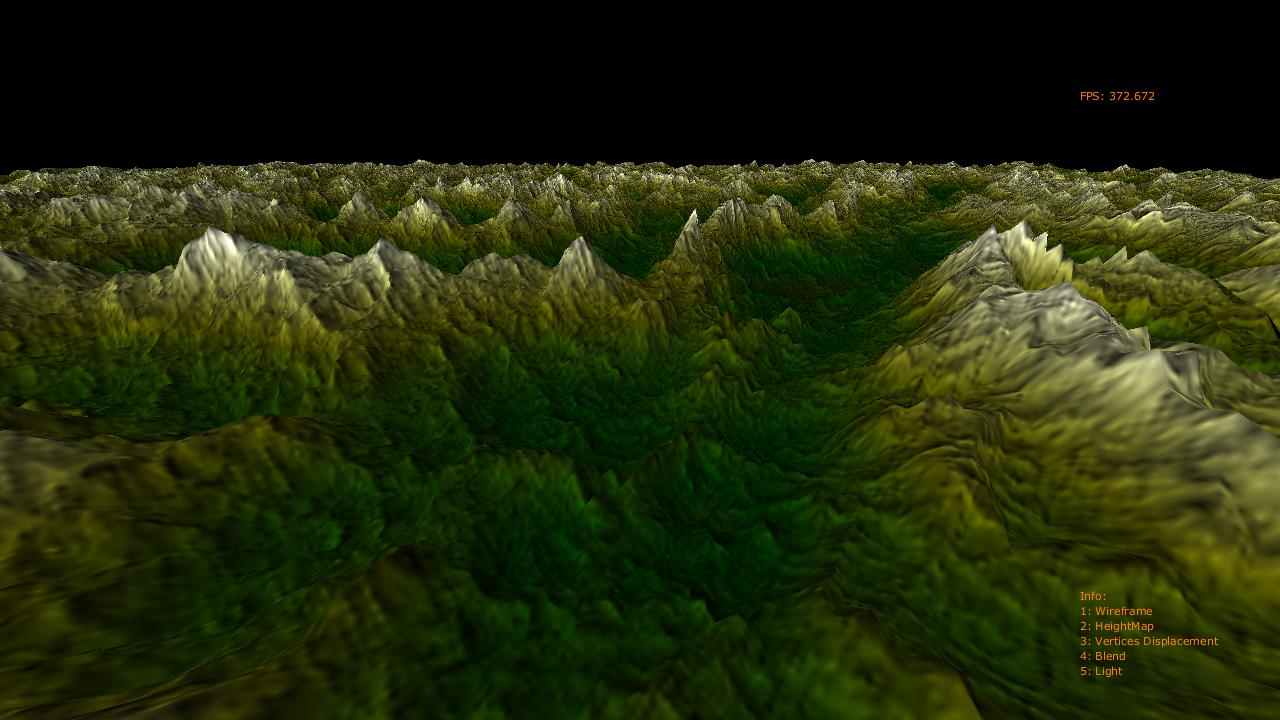
\includegraphics[width=0.5\linewidth]{img/caps/luz.png}}
	\caption{\label{fig:luz} Mapa de altura aplicado a um quadrado, deslocando a altura, com texturas, e ilumina��o.}
\end{figure}

Um v�deo demonstrando a navega��o pelo terreno pode ser visto em \cite{youtube}.


\section{Testes de Desempenho}
\label{testes}
Alguns testes foram feitos para avaliar a velocidade de gera��o dos terrenos com a altera��o de alguns par�metros, utilizando tanto a GPU quanto a CPU. Eles foram executados em um \emph{Core 2 Duo E7400}, com 2GB de mem�ria \emph{RAM} e placa de v�deo \emph{ATI Radeon HD 4850} com 512MB de mem�ria \emph{RAM}, e \emph{driver} vers�o 8.612. As tabelas com os tempos e as conclus�es dos testes s�o apresentadas a seguir.



\subsection{Tempos de Gera��o do Terreno}
\label{testeGeracao}
Neste teste foi medido o tempo m�dio gasto com a gera��o de terrenos tanto na \emph{GPU} quanto na \emph{CPU}. Os seguintes par�metros foram utilizados:

\begin{itemize}
\item \emph{Octaves}: Vari�vel (4, 8, 12, 16)
\item \emph{Lacunarity}: 2.5
\item Ganho: 0.5
\item \emph{Offset}: 1.0
\item Tamanho da textura: 512
\item N�mero de divis�es dos quadrados: 150
\item Tamanho dos quadrados: 5.0
\item Fator \emph{LOD}: 2
\end{itemize}



\begin{table}[H]
	\begin{center}
		\begin{tabular}{|c|c|c|}
			\hline
			\emph{Octaves} & GPU & CPU \\
			\hline
			4 & 28,7236 & 46,2948\\
			\hline
			8 & 28,7432 & 92,4299\\
			\hline
			16 & 28,7887 & 187,103\\
			\hline
			32 & 30,1095 & 370,841\\
			\hline
		\end{tabular}
		\caption{Tempo m�dio (em ms) de gera��o dos terrenos, com n�mero vari�vel de \emph{octaves}}
		\label{tabela:geracao}
	\end{center}
\end{table}


A Figura \ref{fig:geracao} apresenta os tempos anteriores.
\begin{figure}[H]
	\center{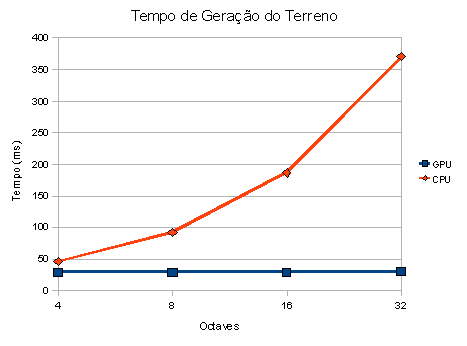
\includegraphics[width=0.4\linewidth]{img/tempoGeracao.png}}
	\caption{\label{fig:geracao} Gr�fico do tempo m�dio (em ms) de gera��o dos terrenos, com n�mero vari�vel de \emph{octaves}.}
\end{figure}


Como pode ser visto, o tempo de gera��o do terreno na \emph{GPU} permanece quase constante, enquanto a gera��o na \emph{CPU} tem um comportamento praticamente linear.


\subsection{\emph{Frames} por Segundo Durante Navega��o}
\label{testeFPS}
Neste teste foi medido o \emph{Frames por segundo} (\sigla{FPS}{Frames por segundo}) m�dio durante a navega��o pelo terreno gerado proceduralmente, por 30 segundos. Os seguintes par�metros foram utilizados:

\begin{itemize}
\item \emph{Octaves}: 16
\item \emph{Lacunarity}: 2.5
\item Ganho: 0.5
\item \emph{Offset}: 1.0
\item Tamanho da textura: 512
\item N�mero de divis�es dos quadrados: 150
\item Tamanho dos quadrados: 5.0
\item Fator \emph{LOD}: 2
\end{itemize}

A Tabela \ref{tabela:fps} mostra os tempos m�dios, m�nimos e a m�dia de \emph{FPS}. Al�m disso, h� o n�mero de \emph{frames} renderizados durante o percurso:

\begin{table}[H]
	\begin{center}
		\begin{tabular}{|c|c|c|c|c|}
			\hline
			 & Total de \emph{Frames} & \emph{FPS} M�nimo & \emph{FPS} M�ximo & \emph{FPS} M�dio \\
			\hline
			CPU & 9664 & 248 & 397 & 322.133\\
			\hline
			GPU & 11287 & 361 & 394 & 376.233\\
			\hline
		\end{tabular}
		\caption{Dados sobre a navega��o pelo mundo durante 30 segundos}
		\label{tabela:fps}
	\end{center}
\end{table}


A Figura \ref{fig:fps} apresenta os tempos anteriores:
\begin{figure}[H]
	\center{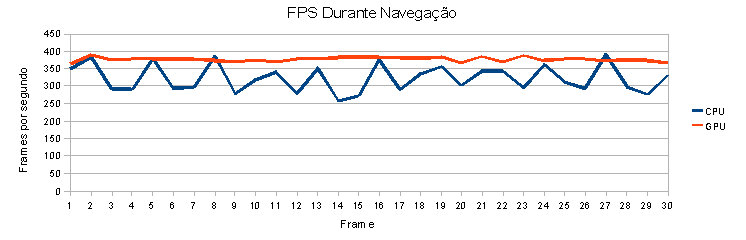
\includegraphics[width=0.9\linewidth]{img/tempoFPS.png}}
	\caption{\label{fig:fps} Gr�fico com o FPS na navega��o pelo mundo durante 30 segundos.}
\end{figure}


Como pode ser visto atrav�s do gr�fico, a navega��o pelo mundo, utilizando a gera��o dos terrenos na GPU, � muito mais fluida, sem quedas bruscas de \emph{FPS}, como nos \emph{frames} 3, 6, 9, 12, 14, 17, 20, 23, 26 e 29, gra�as �s centenas de unidades de processamento presentes na GPU.

Na gera��o pela CPU, tais quedas correspondem justamente aos momentos em que o sistema gera novos terrenos e podem significar um menor senso de imers�o do usu�rio no mundo virtual.



% ********** REFERÊNCIAS **********
%\bibliographystyle{abnt-alf}	 % Existem ainda: abbrv, acm, alpha, amsalpha, amsplain
\nocite{*}
\bibliographystyle{abnt-num}
\bibliography{proposta} % o nome do arquivo .bib com as referências
%\include{bibliografia}															

% \chapter{Entrada de Símbolos e Siglas}
% \par Para fazer a entrada de um símbolo, $\backslash$símbolo\{\simbolo{$\sigma$}{Descrição}\} \{Descriçao\} é a forma % correta. E, para definir uma sigla, $\backslash$sigla\{\sigla{ABNT}{Associação Brasileira de Normas Técnicas}\} % \{Descrição\} deve ser utilizado.
%  \par Obs.: Quando a sigla ou o símbolo aparecerem novamente no texto, não repita o comando, para que a sigla ou símbolo não se repita na lista correspondente.

% *********** APÊNDICES ***********
% ** Condicionados à necessidade **
% \apendice
% \chapter{Primeiro apêndice}
% \par Apêndices são textos elaborados pelo autor a fim de complementar sua argumentação.

% ************ ANEXOS *************
% ** Condicionados à necessidade **
% \anexo
% \chapter{Primeiro anexo}
% \par Anexos são documentos não elaborados pelo autor, que servem de fundamentação, comprovação ou ilustração.

\end{document}

% Quando o número de apêndices ou anexos vier a ser suficiente, é recomendado fazer um sumário separado para os apêndices, localizados imediatamente antes dos apêndices ou anexos. Nesse caso, no sumário principal, apenas é feito referência a este sumário específico.
